
\begin{figure}[!htbp]
    \begin{centering}
        \subfloat[Loading time in minutes for 25kb matrix]
        {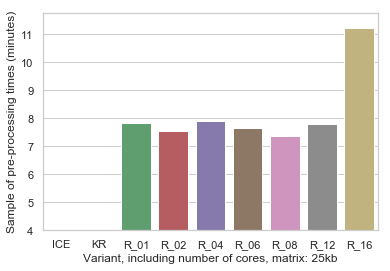
\includegraphics[scale=0.9]{figures/results/loadtimes_25}} \\
        % \caption[Correction time of 25kb]
        % {\textbf{Runtime in minutes} for correcting the 25kb matrix.}
        \subfloat[Loading time in minutes for 50kb matrix]
        {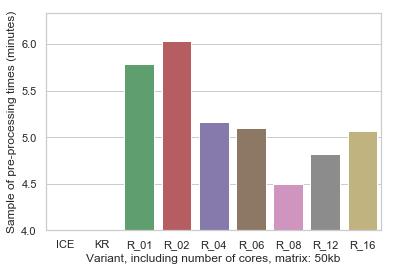
\includegraphics[scale=0.9]{figures/results/loadtimes_50}}
        \caption[Matrix loading times]
        {\textbf{Matrix loading times} for the different matrix sizes. Even though
        the operations are the same during pre-processing, actual times fluctuated.
        No data is available for ICE and KR variants, however as the pre-processing
        is the same, their values can be thought to be in the same range as the
        others. Equal is better.}
    \label{fig:loadtimes}
    \end{centering}
\end{figure}


